\section{Zielsetzung}
\label{sec:Zielsetzung}

Ziel des Versuches ist es, die effektive Masse der Leitungselektronen in n-dotiertem Galliumarsenid (n-GaAs)
mit Hilfe des Faraday-Effekts zu bestimmen.

\section{Theorie}
\label{sec:Theorie}

\begin{figure}[H]
    \centering
    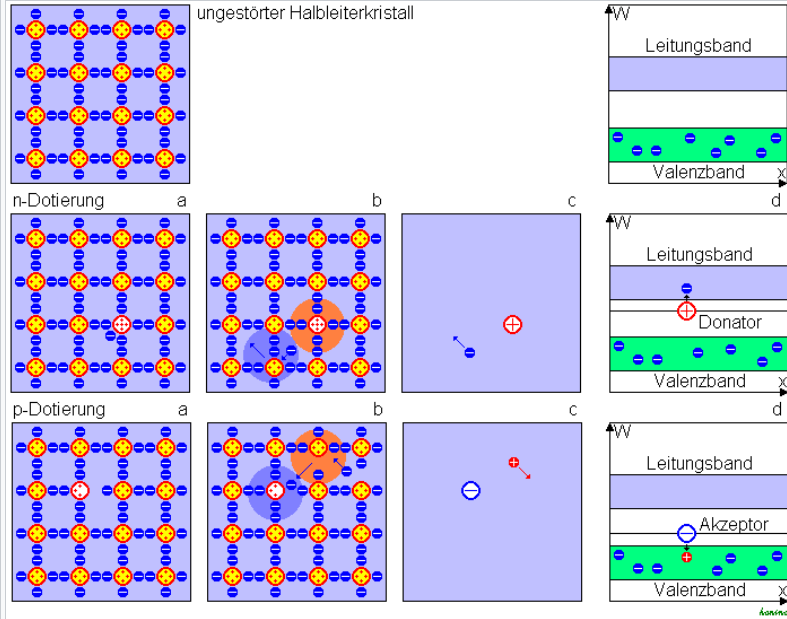
\includegraphics[scale=0.35]{Abbildungen/Dotierung.png}
    \caption{Schematischer Aufbau des Versuchs.\cite{Dotierung}}
    \label{fig:aufbau}
\end{figure}


\begin{figure}[H]
    \centering
    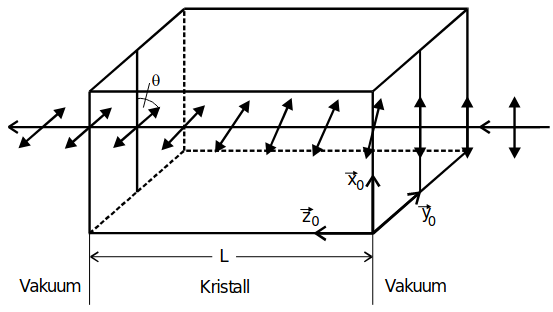
\includegraphics[scale=0.35]{Abbildungen/Doppelbrechung.png}
    \caption{Schematischer Aufbau des Versuchs.\cite{V46_Anhang}}
    \label{fig:aufbau}
\end{figure}